\DiaryEntry{Inside Interesting Integrals, 1 (Section 1.5, even/odd Functions)}{2016-02-09}{Integrals}

Based on \cite{nahin2020inside}, Section 1.5. Consider the integral

\bee
\int_{-1}^1 g(x) dx = \int_{-1}^1 \frac{\cos x}{d(x)+1} dx
\eee

with a general function $d(x)$. We can split the integrand into an even and odd part which are defined according to

\bee
g_e(x) = \frac{g(x) + g(-x)}{2}
\eee

and

\bee
g_o(x) = \frac{g(x) - g(-x)}{2}
\eee

We can express the function in terms of even and odd part according to

\bee
g(x) = g_e(x) + g_o(x)
\eee

The even and odd part have the following properties,

\bee
g_e(x) = g_e(-x), \quad g_o(x) = -g_o(-x)
\eee

From the second condition, we see that $g_o(0) = 0$. When the integration bounds are symmetric, the integral of the odd function $g_o(x)$ becomes zero,

\bee
\int_{-A}^A g_o(x) dx = 0
\eee

and the integral $\int_{-1}^1 g(x) dx$ therefore reduces to an integral over the even part,

\[
\int_{-1}^1 g(x) dx = \int_{-1}^1 g_e(x) dx
\]

The even part $g_e(x)$ may be simpler to integrate than $g(x)$. Next, we calculate the even part of $g(x)$,

\bee
g_e(x) = \frac{1}{2} \left[ \frac{\cos(x)}{d(x) + 1} + \frac{\cos(x)}{d(-x) + 1}\right] = \frac{\cos(x)}{2}  \frac{2 + d(-x) + d(x)}{ 1 + d(x) + d(-x) + d(x)d(-x) }
\eee

This does not look much easier; however, if we put the restriction $d(x)d(-x) = 1$ on $d(x)$, then things become very simple,

\bee
g_e(x) = \frac{\cos(x)}{2}  \frac{2 + d(-x) + d(x)}{ 2 + d(x) + d(-x) } = \frac{\cos(x)}{2}
\eee

Integrating this expression finally yields

\bee
\int_{-1}^1 g(x) dx = \int_{-1}^1 g_o(x) + g_e(x) dx = \int_{-1}^1 g_e(x) dx = \int_{-1}^1 \frac{\cos(x)}{2} dx = \sin(1)
\eee

For fun, we can choose $d(x) = e^x$ (the condition on $d(x)$ holds as $d(x)d(-x) = e^x e^{-x} = 1$) and check this against Maxima,

\begin{verbatim}
(%i1)	gx:cos(x)/(exp(-x)+1);
(%o1)	cos(x)/(%e^(-x)+1)
(%i2)	gmx:subst(-x, x, gx);
(%o2)	cos(x)/(%e^x+1)
(%i3)	ge:ratsimp((gx+gmx)/2);
(%o3)	cos(x)/2
(%i4)	go:ratsimp((gx-gmx)/2);
(%o4)	((%e^x-1)*cos(x))/(2*%e^x+2)
(%i5)	integrate(go, x, -1, 1);
(%o5)	0
(%i6)	integrate(ge, x, -1, 1);
(%o6)	sin(1)
\end{verbatim}

Next we plot the involved functions. The function $g(x)$ is in blue, the even part $g_e(x)$ is red, and the odd part $g_o(x)$ is in green.

\begin{figure}[H]
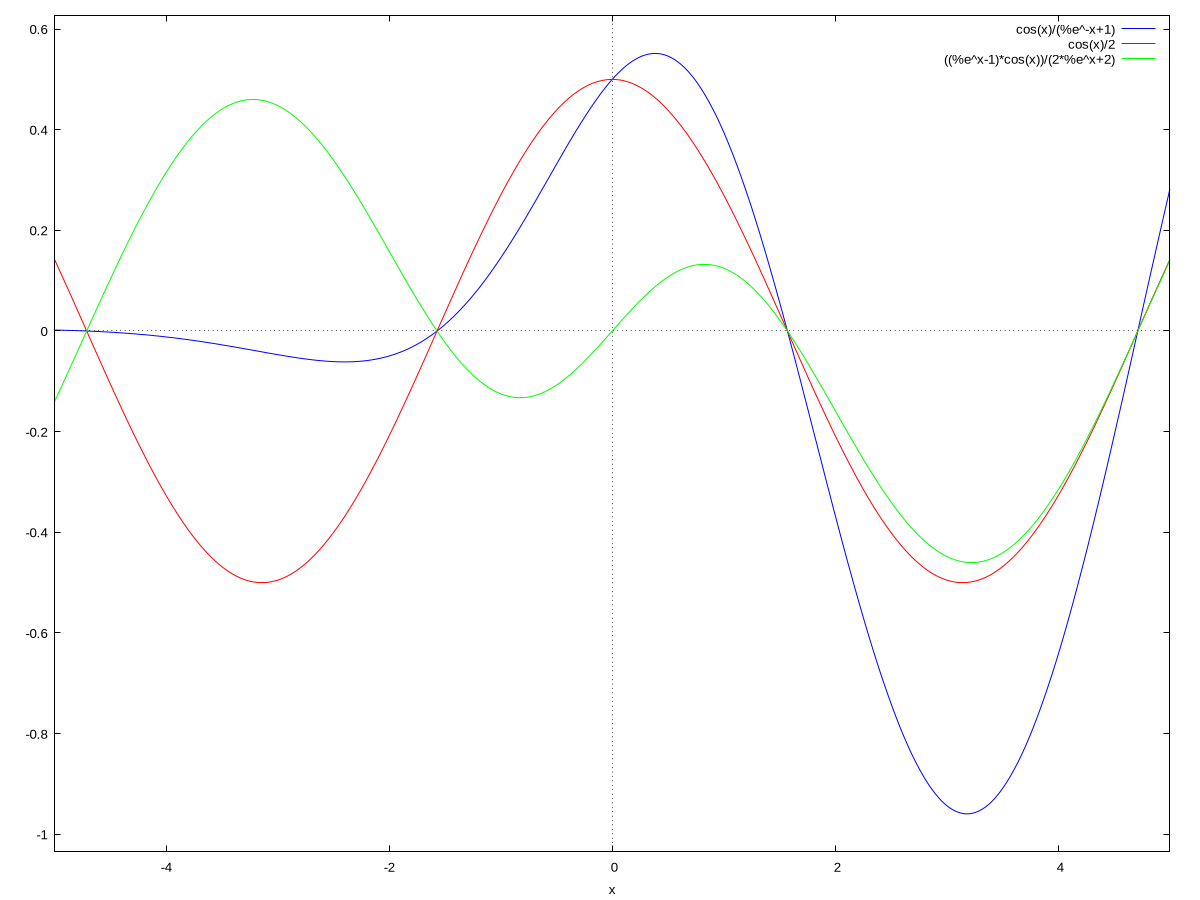
\includegraphics[scale=0.3]{images/2016-02-09_plot_1.png}
\end{figure}





%%% Local Variables:
%%% mode: latex
%%% TeX-master: "journal"
%%% End:
